% !TeX program = xelatex
\documentclass[a4paper,10pt]{article}

% ============================================================================
% កញ្ចប់បណ្ណាល័យ (Packages) – អនុវិទ្យាល័យព្រះក្រសាំង (គ្មាន LCD / សន្លឹកកិច្ចការជាគោល)
% ============================================================================
\usepackage[a4paper, left=0.95cm, right=0.95cm, top=0.85cm, bottom=0.92cm, footskip=0.52cm]{geometry}
\usepackage{amsmath}
\usepackage{unicode-math}
\usepackage{fontspec}
\usepackage{array, longtable, multirow, colortbl}
\usepackage[table]{xcolor}
\usepackage{enumitem}
\usepackage{pifont}
\usepackage{fancyhdr}
\usepackage{tikz}
\usetikzlibrary{calc, arrows.meta, decorations.pathreplacing, patterns, positioning, babel}

\makeatletter
\let\@expl@@@mark@update@singlecol@structures@@\relax
\makeatother

% ============================================================================
% ការកំណត់ពុម្ពអក្សរ (Cross-Platform Windows + Linux Cloud fonts/)
% ============================================================================
\providecommand{\NGSFindFonts}{%
  \IfFileExists{C:/Windows/Fonts/cambria.ttc}{%
    \def\NGSSysPath{C:/Windows/Fonts/}%
    \def\NGSUserPath{C:/Users/KIT/AppData/Local/Microsoft/Windows/Fonts/}%
  }{%
    \IfFileExists{./fonts/KhmerOSsiemreap.ttf}{\def\NGSSysPath{./fonts/}\def\NGSUserPath{./fonts/}}{%
    \IfFileExists{../fonts/KhmerOSsiemreap.ttf}{\def\NGSSysPath{../fonts/}\def\NGSUserPath{../fonts/}}{%
    \IfFileExists{../../fonts/KhmerOSsiemreap.ttf}{\def\NGSSysPath{../../fonts/}\def\NGSUserPath{../../fonts/}}{%
    \IfFileExists{../../../fonts/KhmerOSsiemreap.ttf}{\def\NGSSysPath{../../../fonts/}\def\NGSUserPath{../../../fonts/}}{%
    \IfFileExists{../../../../fonts/KhmerOSsiemreap.ttf}{\def\NGSSysPath{../../../../fonts/}\def\NGSUserPath{../../../../fonts/}}{%
    \IfFileExists{../../../../../fonts/KhmerOSsiemreap.ttf}{\def\NGSSysPath{../../../../../fonts/}\def\NGSUserPath{../../../../../fonts/}}{%
    \IfFileExists{../../../../../../fonts/KhmerOSsiemreap.ttf}{\def\NGSSysPath{../../../../../../fonts/}\def\NGSUserPath{../../../../../../fonts/}}{%
      \def\NGSSysPath{../../../../../../../fonts/}\def\NGSSysPath{../../../../../../../fonts/}\def\NGSUserPath{../../../../../../../fonts/}%
    }}}}}}}%
  }%
}
\NGSFindFonts

\setmathfont[
  Path={\NGSSysPath},
  FontIndex=1,
  Scale=1.02
]{cambria.ttc}

\defaultfontfeatures{Ligatures=TeX}

\setmainfont[
  Path={\NGSUserPath},
  Extension=.ttf,
  Script=Khmer,
  BoldFont={KhmerOSsiemreap},
  BoldFeatures={FakeBold=1.8},
  ItalicFont={KhmerOSsiemreap},
  ItalicFeatures={FakeSlant=0.25},
  BoldItalicFont={KhmerOSsiemreap},
  BoldItalicFeatures={FakeBold=1.8, FakeSlant=0.25}
]{KhmerOSsiemreap}

\newfontfamily\muol[
  Path={\NGSUserPath},
  Extension=.ttf,
  Script=Khmer
]{KhmerOSmuollight}

\newfontfamily\TimesEn[
  Path={\NGSSysPath},
  Extension=.ttf,
  Scale=1.00,
  BoldFont={timesbd},
  ItalicFont={timesi},
  BoldItalicFont={timesbi}
]{times}

\newfontfamily\NagaBold[
  Path={\NGSUserPath},
  Extension=.ttf
]{AKbalthom Naga Bold}

\newfontfamily\CalibriFont[
  Path={\NGSSysPath},
  Extension=.ttf
]{calibri}

\newfontfamily\Tacteing[
  Path={\NGSUserPath}
]{TACTENG.TTF}

\newfontfamily\CourierBullet[
  Path={\NGSSysPath},
  Extension=.ttf
]{cour}
\newcommand{\wcirc}{{\CourierBullet\fontsize{9.5pt}{11pt}\selectfont o}}

\XeTeXlinebreaklocale "km"
\XeTeXlinebreakskip = 0pt plus 1pt minus 0.1pt

% ============================================================================
% ការកំណត់ពណ៌ និងទម្រង់ទំព័រ (Colors & Page Style)
% ============================================================================
\definecolor{stepgray}{HTML}{D9D9D9}
\definecolor{headgray}{HTML}{F2F2F2}
\definecolor{boxgray}{HTML}{D9D9D9}
\definecolor{darkred}{HTML}{C00000}
\definecolor{red5e}{HTML}{FF0000}

\pagestyle{fancy}
\fancyhf{}
\renewcommand{\headrulewidth}{0pt}
\fancyfoot[R]{\CalibriFont\fontsize{11pt}{13pt}\selectfont\thepage}

\setlength{\parindent}{0pt}
\setlength{\parskip}{0pt}
\setlength{\tabcolsep}{3.8pt}

\newcolumntype{L}[1]{>{\raggedright\arraybackslash}p{#1}}

% ============================================================================
% ម៉ាក្រូជំនួយ (Helper Macros)
% ============================================================================
\newcommand{\en}[1]{{\TimesEn #1}}
\newcommand{\enbf}[1]{{\TimesEn\textbf{#1}}}
\newcommand{\unit}[1]{\,\text{\en{#1}}}
\newcommand{\riel}{\,\text{៛}}
\newcommand{\usd}{\,\text{\en{\$}}}
\newcommand{\fiveE}[1]{{\NagaBold\fontsize{9.5pt}{13pt}\selectfont\textcolor{red5e}{#1}}}
\newcommand{\timenote}[1]{\textcolor{darkred}{\textit{#1}}}
\newcommand{\redsub}[1]{\textcolor{darkred}{#1}}
\newcommand{\graybox}[1]{\colorbox{boxgray}{\strut\hspace{2pt}#1\hspace{2pt}}}
\newcommand{\ditem}{\tikz[baseline=-0.5ex]\fill (0,0.42ex) -- (0.42ex,0) -- (0,-0.42ex) -- (-0.42ex,0) -- cycle;\hspace{0.3em}}
\newcommand{\cnum}[1]{{\fontsize{10.5pt}{12pt}\selectfont\ding{\numexpr181+#1\relax}}\hspace{0.15em}}
\newcommand{\cfig}[1]{\par\vspace{3pt}{\centering #1\par}\vspace{3pt}}
\newcommand{\stepheader}[1]{\multicolumn{3}{|c|}{\cellcolor{stepgray}\muol #1} \\* \noalign{\hrule height 0.4pt}}
\newcommand{\fboxb}[1]{\begingroup\setlength{\fboxsep}{1.5pt}\fbox{#1}\endgroup}
\newcommand{\khmflourish}{{\Tacteing\fontsize{36pt}{14pt}\selectfont\raisebox{-5pt}{3}}}

% ============================================================================
% ម៉ាក្រូគូសរូប TikZ ស-ខ្មៅ ១០០% (x=1cm, y=1cm, font=\scriptsize, width=7.55cm)
% ============================================================================

% ១. E1 Engage: បេសកកម្មអ្នកលក់ផ្លែស្វាយ (ស្ទង់អន្ទាក់ភាគបែងថ្លៃដើម vs ថ្លៃលក់)
\newcommand{\figEngagePCTThreeTwoOne}{%
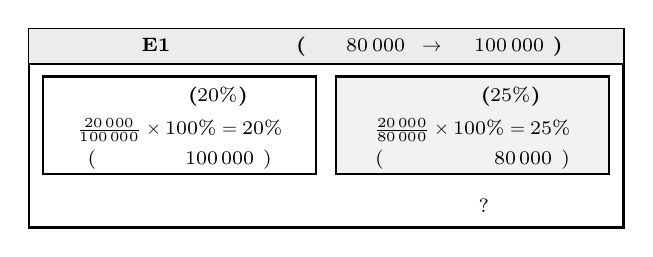
\begin{tikzpicture}[x=1cm, y=1cm, every node/.style={font=\scriptsize, text=black}]
  \draw[black, line width=0.9pt] (0,0) rectangle (7.55,2.52);
  \fill[gray!15] (0,2.08) rectangle (7.55,2.52);
  \draw[black, line width=0.6pt] (0,2.08) -- (7.55,2.08);
  \node at (3.775,2.30) {\textbf{បេសកកម្ម \en{E1}៖ លក់ស្វាយ ១ កន្ត្រក (ទិញដើម $80\,000\riel$ $\to$ លក់ $100\,000\riel$)}};

  \draw[black, line width=0.8pt] (0.18,0.68) rectangle (3.65,1.92);
  \node at (1.915,1.66) {\textbf{គំនិតសិស្ស ក ($20\%$)}};
  \node at (1.915,1.24) {$\frac{20\,000}{100\,000}\times 100\% = 20\%$};
  \node at (1.915,0.86) {(ធៀបនឹង\textbf{ប្រាក់លក់} $100\,000\riel$)};

  \draw[black, line width=0.85pt, fill=gray!10] (3.90,0.68) rectangle (7.37,1.92);
  \node at (5.635,1.66) {\textbf{គំនិតសិស្ស ខ ($25\%$)}};
  \node at (5.635,1.24) {$\frac{20\,000}{80\,000}\times 100\% = 25\%$};
  \node at (5.635,0.86) {(ធៀបនឹង\textbf{ប្រាក់ថ្លៃដើម} $80\,000\riel$)};

  \node at (3.775,0.28) {\textbf{សំណួរគន្លឹះ៖} ភាគរយប្រាក់ចំណេញ ត្រូវធៀបនឹង\textbf{ថ្លៃលក់} ឬ\textbf{ថ្លៃដើម}?};
\end{tikzpicture}}

% ២. E2 Act 1: បន្ទះភាគរយមាត្រដ្ឋានទ្វេ 100% (សិស្សជាប់តេស្ត 30 នាក់ ក្នុង 40 នាក់ ទំ.៣២)
\newcommand{\figPercentBarPCTThreeTwoOne}{%
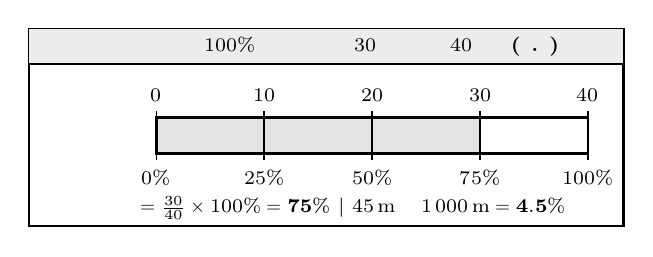
\begin{tikzpicture}[x=1cm, y=1cm, every node/.style={font=\scriptsize, text=black}]
  \draw[black, line width=0.9pt] (0,0) rectangle (7.55,2.50);
  \fill[gray!15] (0,2.06) rectangle (7.55,2.50);
  \draw[black, line width=0.6pt] (0,2.06) -- (7.55,2.06);
  \node at (3.775,2.28) {\textbf{បន្ទះមាត្រដ្ឋានទ្វេ $100\%$៖ សិស្សប្រឡងជាប់ $30$ នាក់ ក្នុង $40$ នាក់ (ទំ.៣២)}};

  % Bar from x=1.62 to x=7.10 (length 5.48 cm; each 25% = 1.37 cm)
  \fill[gray!22] (1.62,0.92) rectangle (5.73,1.38);
  \draw[black, line width=0.85pt] (1.62,0.92) rectangle (7.10,1.38);
  \foreach \x/\s/\p in {1.62/0/0\%, 2.99/10/25\%, 4.36/20/50\%, 5.73/30/75\%, 7.10/40/100\%} {
    \draw[black, line width=0.65pt] (\x,0.84) -- (\x,1.46);
    \node[above=0.5pt] at (\x,1.44) {$\s$};
    \node[below=0.5pt] at (\x,0.86) {$\p$};
  }
  \node[anchor=west] at (0.14,1.62) {\textbf{ចំនួនសិស្ស៖}};
  \node[anchor=west] at (0.14,0.68) {\textbf{ភាគរយ៖}};
  \node at (3.775,0.23) {$\text{ភាគរយជាប់} = \frac{30}{40}\times 100\% = \mathbf{75\%}$ \en{|} $45\unit{m}$ នៃ $1\,000\unit{m} = \mathbf{4.5\%}$};
\end{tikzpicture}}

% ៣. E2 Act 2: បន្ទះប្រៀបធៀប ប្រាក់ចំណេញ និង ប្រាក់ខាត (ប្រាក់ថ្លៃដើម = 100% ជានិច្ច)
\newcommand{\figProfitLossBarPCTThreeTwoOne}{%
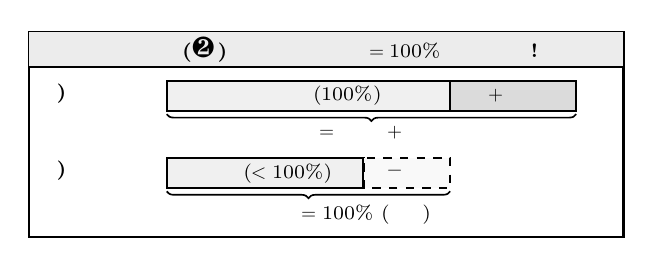
\begin{tikzpicture}[x=1cm, y=1cm, every node/.style={font=\scriptsize, text=black}]
  \draw[black, line width=0.9pt] (0,0) rectangle (7.55,2.60);
  \fill[gray!15] (0,2.16) rectangle (7.55,2.60);
  \draw[black, line width=0.6pt] (0,2.16) -- (7.55,2.16);
  \node at (3.775,2.38) {\textbf{គោលការណ៍មាស (\cnum{2})៖ គូសរង្វង់ប្រាក់ថ្លៃដើម $= 100\%$ ជាភាគបែងជានិច្ច!}};

  % ករណីចំណេញ
  \node[anchor=west] at (0.16,1.82) {\textbf{១) ចំណេញ៖}};
  \draw[black, line width=0.8pt, fill=gray!12] (1.75,1.60) rectangle (5.35,1.98);
  \node at (3.55,1.79) {ប្រាក់ថ្លៃដើម ($100\%$)};
  \draw[black, line width=0.8pt, fill=gray!28] (5.35,1.60) rectangle (6.95,1.98);
  \node at (6.15,1.79) {$+$ ចំណេញ};
  \draw[decorate, decoration={brace, mirror, amplitude=2.5pt}, line width=0.6pt] (1.75,1.56) -- (6.95,1.56);
  \node at (4.35,1.32) {ថ្លៃលក់ $=$ ថ្លៃដើម $+$ ប្រាក់ចំណេញ};

  % ករណីខាត
  \node[anchor=west] at (0.16,0.84) {\textbf{២) ខាត៖}};
  \draw[black, line width=0.8pt, fill=gray!12] (1.75,0.62) rectangle (4.25,1.00);
  \node at (3.00,0.81) {ថ្លៃលក់ ($<100\%$)};
  \draw[black, line width=0.8pt, dashed, fill=gray!5] (4.25,0.62) rectangle (5.35,1.00);
  \node at (4.80,0.81) {$-$ ខាត};
  \draw[decorate, decoration={brace, mirror, amplitude=2.5pt}, line width=0.6pt] (1.75,0.58) -- (5.35,0.58);
  \node at (3.55,0.28) {ប្រាក់ថ្លៃដើមទាំងមូល $= 100\%$ (ភាគបែង)};
\end{tikzpicture}}

% ៤. E4 Elaborate: ខ្សែសង្វាក់លក់រថយន្តពីរដំណាក់កាល (Shifting Reference Base ទំ.៣២-៣៣)
\newcommand{\figElaborateCarChainPCTThreeTwoOne}{%
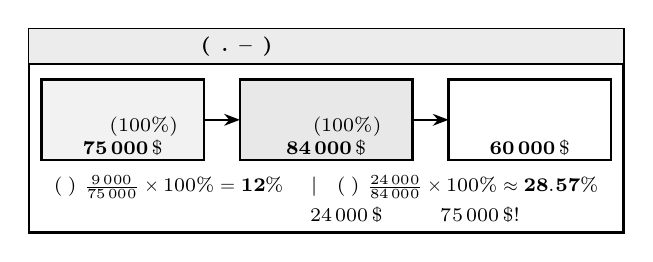
\begin{tikzpicture}[x=1cm, y=1cm, every node/.style={font=\scriptsize, text=black}]
  \draw[black, line width=0.9pt] (0,0) rectangle (7.55,2.58);
  \fill[gray!15] (0,2.14) rectangle (7.55,2.58);
  \draw[black, line width=0.6pt] (0,2.14) -- (7.55,2.14);
  \node at (3.775,2.36) {\textbf{លំហាត់គំរូ (ទំ.៣២--៣៣)៖ ការផ្លាស់ប្ដូរប្រាក់ថ្លៃដើមតាមម្ចាស់នីមួយៗ}};

  % Box 1: Company
  \draw[black, line width=0.85pt, fill=gray!10] (0.16,0.92) rectangle (2.22,1.94);
  \node at (1.19,1.68) {\textbf{ក្រុមហ៊ុននាំចូល}};
  \node at (1.19,1.34) {ដើមទី ១ ($100\%$)៖};
  \node at (1.19,1.08) {$\mathbf{75\,000\usd}$};

  % Arrow 1
  \draw[-{Stealth[length=2mm]}, line width=0.85pt] (2.22,1.43) -- (2.68,1.43);

  % Box 2: Mr. Ly Srun
  \draw[black, line width=1.0pt, fill=gray!18] (2.68,0.92) rectangle (4.87,1.94);
  \node at (3.775,1.68) {\textbf{លោកលីស្រ៊ុន}};
  \node at (3.775,1.34) {ដើមទី ២ ($100\%$)៖};
  \node at (3.775,1.08) {$\mathbf{84\,000\usd}$};

  % Arrow 2
  \draw[-{Stealth[length=2mm]}, line width=0.85pt] (4.87,1.43) -- (5.33,1.43);

  % Box 3: Mr. Heng Lim
  \draw[black, line width=0.85pt] (5.33,0.92) rectangle (7.39,1.94);
  \node at (6.36,1.68) {\textbf{លោកហេងលីម}};
  \node at (6.36,1.34) {ទិញបន្តថ្លៃ៖};
  \node at (6.36,1.08) {$\mathbf{60\,000\usd}$};

  \node at (3.775,0.58) {(ក) $\frac{9\,000}{75\,000}\times 100\% = \mathbf{12\%}$ \quad\en{|}\quad (ខ) $\frac{24\,000}{84\,000}\times 100\% \approx \mathbf{28.57\%}$};
  \node at (3.775,0.22) {\textbf{ប្រយ័ត្នអន្ទាក់៖} កុំយកប្រាក់ខាត $24\,000\usd$ ទៅចែកនឹង $75\,000\usd$!};
\end{tikzpicture}}

% ៥. E5 Evaluate: ជម្រើសវិនិច្ឆ័យ A-D
\newcommand{\figExitPCTThreeTwoOne}{%
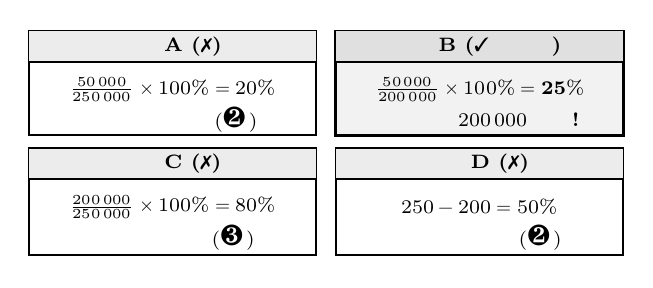
\begin{tikzpicture}[x=1cm, y=1cm, every node/.style={font=\scriptsize, text=black}]
  % A
  \draw[black, line width=0.8pt] (0,1.52) rectangle (3.65,2.84);
  \fill[gray!15] (0,2.45) rectangle (3.65,2.84);
  \draw[black, line width=0.55pt] (0,2.45) -- (3.65,2.45);
  \node at (1.825,2.645) {\textbf{ជម្រើស \en{A} (\ding{55})}};
  \node at (1.825,2.10) {$\frac{50\,000}{250\,000}\times 100\% = 20\%$};
  \node at (1.825,1.72) {ច្រឡំយកថ្លៃលក់ជាភាគបែង (\cnum{2})};

  % B (Correct)
  \draw[black, line width=1.1pt, fill=gray!10] (3.90,1.52) rectangle (7.55,2.84);
  \fill[gray!24] (3.90,2.45) rectangle (7.55,2.84);
  \draw[black, line width=0.6pt] (3.90,2.45) -- (7.55,2.45);
  \node at (5.725,2.645) {\textbf{ជម្រើស \en{B} (\ding{51} ត្រឹមត្រូវ)}};
  \node at (5.725,2.10) {$\frac{50\,000}{200\,000}\times 100\% = \mathbf{25\%}$};
  \node at (5.725,1.72) {\textbf{ធៀបនឹងថ្លៃដើម $200\,000\riel$ ត្រូវ!}};

  % C
  \draw[black, line width=0.8pt] (0,0) rectangle (3.65,1.35);
  \fill[gray!15] (0,0.96) rectangle (3.65,1.35);
  \draw[black, line width=0.55pt] (0,0.96) -- (3.65,0.96);
  \node at (1.825,1.155) {\textbf{ជម្រើស \en{C} (\ding{55})}};
  \node at (1.825,0.61) {$\frac{200\,000}{250\,000}\times 100\% = 80\%$};
  \node at (1.825,0.22) {មិនបានដករកប្រាក់ចំណេញ (\cnum{3})};

  % D
  \draw[black, line width=0.8pt] (3.90,0) rectangle (7.55,1.35);
  \fill[gray!15] (3.90,0.96) rectangle (7.55,1.35);
  \draw[black, line width=0.55pt] (3.90,0.96) -- (7.55,0.96);
  \node at (5.725,1.155) {\textbf{ជម្រើស \en{D} (\ding{55})}};
  \node at (5.725,0.61) {$250 - 200 = 50\%$};
  \node at (5.725,0.22) {ច្រឡំប្រាក់ពិតជាភាគរយ (\cnum{2})};
\end{tikzpicture}}

% ============================================================================
% ចាប់ផ្ដើមឯកសារ (Document Body)
% ============================================================================
\begin{document}
\fontsize{10pt}{15.2pt}\selectfont

% -------------------- ក្បាលកិច្ចតែងការ (Header) --------------------
\begin{center}
  {\muol\fontsize{11pt}{16pt}\selectfont ព្រះរាជាណាចក្រកម្ពុជា}\\[2pt]
  {\muol\fontsize{10pt}{15pt}\selectfont ជាតិ សាសនា ព្រះមហាក្សត្រ}\\[1pt]
  \khmflourish
\end{center}

\vspace{-24pt}
{\muol\fontsize{9.5pt}{12.5pt}\selectfont
មន្ទីរអប់រំ យុវជន និងកីឡា ខេត្តកំពង់ធំ\\
ការិយាល័យអប់រំ យុវជន និងកីឡា ស្រុកកំពង់ស្វាយ\\
អនុវិទ្យាល័យព្រះក្រសាំង}

\vspace{1pt}
\begin{center}
  {\muol\fontsize{10pt}{14pt}\selectfont កិច្ចតែងការបង្រៀន}
\end{center}
\vspace{0pt}

% -------------------- ព័ត៌មានទូទៅ (Metadata) --------------------
{\renewcommand{\arraystretch}{0.98}
\hspace*{3.1cm}%
\begin{tabular}{@{}l l L{11.0cm}@{}}
  - \hspace{0.35cm} មុខវិជ្ជា & : & គណិតវិទ្យា ថ្នាក់ទី៨ (ពីជគណិត) \\
  - \hspace{0.35cm} ចំណងជើងមេរៀន & : & មេរៀនទី៣៖ ទំហំសមាមាត្រនិងភាគរយ \\
  - \hspace{0.35cm} ចំណងជើងរង & : & ២.១–២.២. ភាគរយ ប្រាក់ចំណេញនិងប្រាក់ខាត (ទំ.៣១–៣៣, ៤១–៤២) \\
  - \hspace{0.35cm} រយៈពេល & : & ១ ម៉ោងសិក្សា (៥០ នាទី) \\
  - \hspace{0.35cm} បង្រៀនដោយ & : & ហុក ប៊ុនថែន \\
  - \hspace{0.35cm} កាលបរិច្ឆេទ & : & ថ្ងៃសុក្រ ទី២០ ខែវិច្ឆិកា ឆ្នាំ២០២៦ \\
\end{tabular}

\vspace{2pt}

% -------------------- I. វត្ថុបំណង --------------------
\textbf{I.} {\muol វត្ថុបំណង}\\[1pt]
\hspace*{0.55cm}%
\begin{tabular}{@{}l l L{14.2cm}@{}}
  \wcirc \hspace{0.25cm} វិជ្ជាសម្បទា & : & សិស្សប្រាប់វិធីសរសេរបរិមាណ $a$ មួយជាភាគរយនៃបរិមាណ $b$ មួយទៀត ($\frac{a}{b}\times 100\%$ ក្នុងឯកតាដូចគ្នា) និងប្រាប់រូបមន្តភាគរយប្រាក់ចំណេញនិងប្រាក់ខាតធៀបនឹងប្រាក់ថ្លៃដើម ($100\%$) បានត្រឹមត្រូវ ។ \\
  \wcirc \hspace{0.25cm} បំណិនសម្បទា & : & សិស្សប្ដូរឯកតា គណនាភាគរយនៃបរិមាណ ភាគរយប្រាក់ចំណេញ ភាគរយប្រាក់ខាត និងថ្លៃលក់ក្នុងចំណោទជំនួញជីវភាពពិត (រថយន្តលក់បន្ត និងទោចក្រយានយន្តពូសុខ ទំ.៣១–៣៣) លើសន្លឹកកិច្ចការបានត្រឹមត្រូវ ។ \\
  \wcirc \hspace{0.25cm} ចរិយាសម្បទា & : & សិស្សមានទម្លាប់ផ្ទៀងផ្ទាត់ឯកតា និងកំណត់ប្រាក់ថ្លៃដើមពិតប្រាកដមុនគណនា មានភាពស្មោះត្រង់ក្នុងការលក់ដូរ និងចេះគិតគូរផែនការហិរញ្ញវត្ថុគ្រួសារប្រកបដោយការទទួលខុសត្រូវ ។ \\
\end{tabular}

\vspace{2pt}

% -------------------- II. សម្ភារៈឧបទេស --------------------
\textbf{II.} {\muol សម្ភារៈឧបទេស}\\[1pt]
\hspace*{0.55cm}$\bullet$ \hspace{0.35cm} សៀវភៅសិក្សាគោលថ្នាក់ទី៨ (ទំ.៣១–៣៣, ៤១–៤២) ក្ដារខៀន ដីស/ហ្វឺត បន្ទាត់ត្រង់ និង\textbf{សន្លឹកកិច្ចការសិស្សបំពេញចន្លោះ ស-ខ្មៅ} (\en{Printable\_Materials\_PCT321} ទំព័រ ១–២ សម្រាប់សិស្ស និងទំព័រ ៣ ប្លង់ក្ដារខៀន/ចម្លើយគ្រូ — គ្មានប្រើ \en{LCD})

\vspace{2pt}

% -------------------- III. វិធីសាស្រ្តបង្រៀន --------------------
\textbf{III.} {\muol វិធីសាស្រ្តបង្រៀន}\\[1pt]
\hspace*{0.45cm}%
\begin{tabular}{@{}l l L{14.85cm}@{}}
  $\bullet$ \hspace{0.25cm} គោលវិធី & : & សិស្សមជ្ឈមណ្ឌល (សន្លឹកកិច្ចការបំពេញចន្លោះជាគោល + ការពិភាក្សាជាក្រុមតូច ៣ នាក់) \\
  $\bullet$ \hspace{0.25cm} យុទ្ធវិធីបង្រៀន & : & គំរូស្ថាបនានិយម \en{5Es} រួមបញ្ចូល \textbf{បន្ទះមាត្រដ្ឋានទ្វេ $100\%$ (\en{Dual-Scale Percent Bar})} និង \textbf{ការគូសរង្វង់ប្រាក់ថ្លៃដើមគោល (\en{Reference-Base Circling})} \\
\end{tabular}
}

\vspace{2pt}

% -------------------- IV. ដំណើរការបង្រៀន --------------------
\textbf{IV.} {\muol ដំណើរការបង្រៀន}

\vspace{1pt}
{\renewcommand{\arraystretch}{1.12}
\begin{longtable}{|L{5.50cm}|L{7.90cm}|L{4.80cm}|}
\hline
\multicolumn{1}{|c|}{\cellcolor{headgray}\muol សកម្មភាពគ្រូ} &
\multicolumn{1}{c|}{\cellcolor{headgray}\muol ខ្លឹមសារមេរៀន} &
\multicolumn{1}{c|}{\cellcolor{headgray}\muol សកម្មភាពសិស្ស} \\
\endhead
\hline
\endfoot

% ==================== ជំហានទី១ (2min) ====================
\stepheader{ជំហានទី១ \enbf{(}រដ្ឋបាលថ្នាក់\enbf{)}}
$\bullet$ ពិនិត្យវត្តមាន អនាម័យ និងសណ្ដាប់ធ្នាប់ថ្នាក់រៀន \par
$\bullet$ រៀបចំក្រុមតូច ៣ នាក់តាមតុ និងចែក\textbf{សន្លឹកកិច្ចការសិស្ស (\en{PCT321} ទំព័រ ១–២)}
&
$\bullet$ រដ្ឋបាលថ្នាក់ អនាម័យ និងវិន័យសិក្សា \par
$\bullet$ ចែកសន្លឹកកិច្ចការម្នាក់ ១ សន្លឹក សម្រាប់បំពេញតាមដំណាក់កាល \en{E1--E5}
&
$\circ$ ប្រធានថ្នាក់រាយការណ៍វត្តមានសិស្ស \par
$\circ$ ទទួលសន្លឹកកិច្ចការ សរសេរឈ្មោះ និងអង្គុយតាមក្រុម ៣ នាក់ \\
\hline

% ==================== ជំហានទី២ (9min: កំណែ <=3m + រំលឹក 3m + E1 3m) ====================
\stepheader{ជំហានទី២ \enbf{(}កិច្ចការផ្ទះ \enbf{+} ទំនាក់ទំនងមេរៀនថ្មី\enbf{)}}
\ditem \textbf{កំណែកិច្ចការផ្ទះ ($\le\text{\enbf{3\,min}}$)} \par
$\bullet$ ហៅសិស្ស ២ នាក់ឡើងកែលំហាត់ ទំ.៤១ លេខ ៨ និងលេខ ៩ លើក្ដារខៀន
&
{\centering\redsub{កំណែកិច្ចការផ្ទះមេរៀនមុន (ទំ.៤១ \#8 និង \#9)}\par}
$\bullet$ \textbf{\#8៖} កម្មករថេរ ($25$ នាក់) $\Rightarrow$ ម៉ោងនិងស្បែកជើង\textbf{សមាមាត្រស្រប}៖ $\frac{t}{450}=\frac{26}{1\,300} \implies t = \mathbf{9\unit{h}}$ \par
$\bullet$ \textbf{\#9៖} ផលគុណការងារសរុបថេរ៖ $16 \times x \times 16 = 12 \times 7 \times 8 \implies 256x = 672 \implies x = \mathbf{\frac{21}{8}\unit{h} = 2.625\unit{h}}$
&
$\circ$ ផ្ទៀងចម្លើយ និងកែតម្រូវចូលសៀវភៅកិច្ចការផ្ទះ \\[3pt]

\ditem \textbf{រំលឹកមេរៀនទាក់ទង (\enbf{3min})} \par
$\bullet$ សួររំលឹក៖ «តើ $25\%$ ស្មើនឹងប្រភាគប៉ុន្មាន? ចុះប្រភាគ $\frac{3}{4}$ ប្ដូរជាភាគរយស្មើប៉ុន្មាន?»
&
{\centering\redsub{រំលឹកអត្ថន័យនៃភាគរយ (ថ្នាក់ទី៧)}\par}
$\bullet$ ភាគរយមានន័យថា «ក្នុងមួយរយ»៖ $25\% = \dfrac{25}{100} = \dfrac{1}{4}$ \par
$\bullet$ ប្ដូរប្រភាគទៅជាភាគរយ៖ $\dfrac{3}{4} = \dfrac{3}{4}\times 100\% = \mathbf{75\%}$ ។
&
$\circ$ ឆ្លើយ៖ «$25\% = \frac{25}{100}$ ហើយ $\frac{3}{4}\times 100\% = 75\%$!» \\[3pt]

\fiveE{E1 - Engage (3min)} \timenote{(កុំទាន់ផ្ដល់ចម្លើយ)} \par
\ditem \textbf{បេសកកម្មអ្នកលក់ផ្លែស្វាយ (សន្លឹកកិច្ចការ \en{E1})} \par
$\bullet$ ឱ្យសិស្សអានស្ថានភាពក្នុងប្រអប់ \en{E1} ហើយគូសជ្រើសរើសរវាង \textbf{$20\%$} និង \textbf{$25\%$}
&
\redsub{បេសកកម្ម \en{E1}៖ អ្នកលក់ផ្លែស្វាយនៅផ្សារកំពង់ស្វាយ} \par
មីងសុខាទិញស្វាយ ១ កន្ត្រកថ្លៃដើម $80\,000\riel$ ហើយលក់ចេញបានប្រាក់ $100\,000\riel$ (ចំណេញ $20\,000\riel$) ។ សិស្ស ក ថាចំណេញ $20\%$ ឯសិស្ស ខ ថាចំណេញ $25\%$! \par
$\bullet$ តើសិស្សរូបណាគណនាត្រឹមត្រូវ? ហេតុអ្វី?
&
$\circ$ ពិភាក្សាជាគូ និងគូស \ding{51} ជ្រើសរើសលើសន្លឹកកិច្ចការ \en{E1} \\[3pt]

&
\cfig{\figEngagePCTThreeTwoOne}
& \\
\hline

% ==================== ជំហានទី៣ (17min: E2 11m + E3 6m) ====================
\stepheader{ជំហានទី៣ \enbf{(}ខ្លឹមសារមេរៀនថ្មី\enbf{)}}
\fiveE{E2 - Explore (11min)} \par
$\bullet$ សរសេរចំណងជើងរង \textbf{២. ភាគរយ (២.១ និង ២.២)} លើក្ដារខៀន \par
\ditem \textbf{សកម្មភាព ១៖ ច្រកប្ដូរឯកតា និងបន្ទះភាគរយ (\enbf{5min}, សន្លឹកកិច្ចការ \en{E2-A})} \par
$\bullet$ ដឹកនាំសិស្សពិនិត្យអន្ទាក់ឯកតា $45\unit{m}$ នៃ $1\unit{km}$ (ទំ.៣១) និងលំហាត់គំរូតេស្តសិស្ស $30/40$ (ទំ.៣២)
&
មេរៀនទី៣ \quad {\muol ទំហំសមាមាត្រនិងភាគរយ \enbf{(}ត\enbf{)}} \par
២. ភាគរយ \par
២.១. ការសរសេរបរិមាណមួយជាភាគរយនៃបរិមាណមួយទៀត \par
$\bullet$ \textbf{ឧទាហរណ៍ (ទំ.៣១)៖} សរសេរ $45\unit{m}$ ជាភាគរយនៃ $1\unit{km}$ ៖ \par
\hspace*{0.3cm}ប្ដូរឯកតាជាមុន៖ $1\unit{km} = 1\,000\unit{m} \implies \dfrac{45}{1\,000}\times 100\% = \mathbf{4.5\%}$ \par
$\bullet$ \textbf{លំហាត់គំរូ (ទំ.៣២)៖} តេស្តសិស្ស $40$ នាក់ ជាប់ $30$ នាក់ $\implies \dfrac{30}{40}\times 100\% = \mathbf{75\%}$ ។
&
$\circ$ ប្ដូរ $1\unit{km}=1\,000\unit{m}$ គណនាឃើញ $4.5\%$ និងបំពេញបន្ទះមាត្រដ្ឋានទ្វេ $75\%$ \\[3pt]

&
\cfig{\figPercentBarPCTThreeTwoOne}
& \\[3pt]

\ditem \textbf{សកម្មភាព ២៖ បន្ទះមាត្រដ្ឋានទ្វេ ចំណេញ–ខាត (\enbf{6min}, សន្លឹកកិច្ចការ \en{E2-B})} \par
$\bullet$ ឱ្យសិស្សប្រៀបធៀបករណីចំណេញ និងខាតលើបន្ទះមាត្រដ្ឋានទ្វេ ដោយគូសរង្វង់លើ \textbf{ប្រាក់ថ្លៃដើម $= 100\%$}
&
២.២. ភាគរយប្រាក់ចំណេញនិងប្រាក់ខាត \par
$\bullet$ ពេលលក់ថ្លៃជាងថ្លៃដើម $\to$ \textbf{ចំណេញ} $=$ ថ្លៃលក់ $-$ ប្រាក់ថ្លៃដើម \par
$\bullet$ ពេលលក់ថោកជាងថ្លៃដើម $\to$ \textbf{ខាត} $=$ ប្រាក់ថ្លៃដើម $-$ ថ្លៃលក់ \par
$\bullet$ ទោះចំណេញ ឬខាតក៏ដោយ \textbf{បរិមាណគោល $100\%$ គឺប្រាក់ថ្លៃដើមជានិច្ច!}
&
$\circ$ បំពេញប្រអប់ \en{E2-B} និងគូសរង្វង់ពាក្យ «ប្រាក់ថ្លៃដើម» ជាភាគបែង \\[3pt]

&
\cfig{\figProfitLossBarPCTThreeTwoOne}
& \\[3pt]

% --- E3 Explain (6min) ---
\fiveE{E3 - Explain (6min)} \par
$\bullet$ ដឹកនាំសិស្សបង្គុំប្រអប់\textbf{ជាទូទៅ ២.១} (សៀវភៅគោលទំ.៣២) លើក្ដារខៀន និងសន្លឹកកិច្ចការ \en{E3}
&
$\bullet$ \textbf{ជាទូទៅ ២.១ (ទំ.៣២)៖} ដើម្បីសរសេរបរិមាណ $a$ មួយជាភាគរយនៃបរិមាណ $b$ មួយទៀត (ក្នុងឯកតាដូចគ្នា) គេត្រូវសរសេរ៖ \graybox{$\dfrac{a}{b}\times 100\%$}
&
$\circ$ បំពេញប្រអប់រូបមន្ត ២.១ លើសន្លឹកកិច្ចការ \en{E3} \\[3pt]

$\bullet$ បន្តដឹកនាំសិស្សបង្គុំប្រអប់\textbf{រូបមន្ត ២.២} (សៀវភៅគោលទំ.៣២)
&
$\bullet$ \textbf{រូបមន្ត ២.២ (ទំ.៣២)៖} ភាគរយប្រាក់ចំណេញ ឬប្រាក់ខាតធៀបនឹងប្រាក់ថ្លៃដើម៖ \par
\hspace*{0.3cm}\graybox{$\text{ភាគរយប្រាក់ចំណេញ} = \dfrac{\text{ប្រាក់ចំណេញ}}{\text{ប្រាក់ថ្លៃដើម}}\times 100\%$} \par
\hspace*{0.3cm}\graybox{$\text{ភាគរយប្រាក់ខាត} = \dfrac{\text{ប្រាក់ខាត}}{\text{ប្រាក់ថ្លៃដើម}}\times 100\%$}
&
$\circ$ បំពេញប្រអប់រូបមន្ត ២.២ ទាំងពីរលើសន្លឹកកិច្ចការ \en{E3} \\[3pt]

$\bullet$ ភ្ជាប់\textbf{ធនាគារហេតុផល \cnum{1}--\cnum{4}} សម្រាប់ប្រើក្នុង \en{E4} និង \en{E5}
&
\textbf{ធនាគារហេតុផល (\en{Warrant Bank})៖} \par
\cnum{1} \textbf{ច្រកឯកតាដូចគ្នា៖} ប្ដូរ $a$ និង $b$ ឱ្យមានឯកតាដូចគ្នាមុនសរសេរ $\frac{a}{b}\times 100\%$ \par
\cnum{2} \textbf{គូសរង្វង់ប្រាក់ថ្លៃដើម $= 100\%$៖} ភាគបែងគឺប្រាក់ថ្លៃដើមរបស់ម្ចាស់នោះជានិច្ច \par
\cnum{3} \textbf{ប្រាក់ចំណេញ/ខាត៖} ចំណេញ $=$ លក់ $-$ ដើម \en{|} ខាត $=$ ដើម $-$ លក់ \par
\cnum{4} \textbf{រកថ្លៃលក់៖} ថ្លៃលក់ $= \text{ថ្លៃដើម} + \text{ចំណេញ}$ (ឬ $= \text{ថ្លៃដើម} - \text{ខាត}$)
&
$\circ$ ផ្ទៀងលេខកូដ \cnum{1}--\cnum{4} លើសន្លឹកកិច្ចការ \\
\hline

% ==================== ជំហានទី៤ (20min: E4 10m + E5 10m) ====================
\stepheader{ជំហានទី៤ \enbf{(}ពង្រីកចំណេះដឹង\enbf{)}}
\fiveE{E4 - Elaborate (10min)} \par
\ditem \textbf{លំហាត់គំរូ៖ រថយន្តលក់បន្តពីរដំណាក់កាល (ទំ.៣២–៣៣)} \par
$\bullet$ ឱ្យសិស្សគូសរង្វង់ប្រាក់ថ្លៃដើមតាមម្ចាស់នីមួយៗលើសន្លឹកកិច្ចការ \en{E4} មុនគណនា (ក) និង (ខ)
&
{\muol លំហាត់គំរូ} \textbf{(ទំ.៣២–៣៣ — ក្រុមហ៊ុននាំចូលរថយន្ត)៖} \par
ក្រុមហ៊ុនទិញរថយន្តថ្លៃដើម $75\,000\usd$ លក់ឱ្យ\mbox{លោកលីស្រ៊ុន}ថ្លៃ $84\,000\usd$ ។ ពីរឆ្នាំក្រោយ \mbox{លោកលីស្រ៊ុន}លក់ឱ្យ\mbox{លោកហេងលីម}ថ្លៃ $60\,000\usd$ ។ \par
$\bullet$ \textbf{ក. ក្រុមហ៊ុន (\cnum{2}, \cnum{3})៖} ថ្លៃដើម $= 75\,000\usd$, ចំណេញ $= 84\,000 - 75\,000 = 9\,000\usd$ \par
\hspace*{0.3cm}$\implies \text{ភាគរយចំណេញ} = \dfrac{9\,000}{75\,000}\times 100\% = \graybox{$12\%$}$ \par
$\bullet$ \textbf{ខ. លោកលីស្រ៊ុន (\cnum{2}, \cnum{3})៖} ថ្លៃដើមគាត់ $= \mathbf{84\,000\usd}$, ខាត $= 84\,000 - 60\,000 = 24\,000\usd$ \par
\hspace*{0.3cm}$\implies \text{ភាគរយខាត} = \dfrac{24\,000}{84\,000}\times 100\% = \dfrac{2}{7}\times 100\% \approx \graybox{$28.57\%$}$
&
$\circ$ គូសរង្វង់ថ្លៃដើម $75\,000\usd$ សម្រាប់ (ក) និង $84\,000\usd$ សម្រាប់ (ខ) រួចគណនាឃើញ $12\%$ និង $28.57\%$ \\[3pt]

&
\cfig{\figElaborateCarChainPCTThreeTwoOne}
& \\[3pt]

$\bullet$ សួរសំណួរឆ្លុះបញ្ចាំង \textbf{\en{EIA Looking-Back} (1min)}
&
\textbf{\en{EIA Looking-Back}៖} «ក្នុងសំណួរ (ខ) ហេតុអ្វីយើងមិនយក $24\,000\usd$ ទៅចែកនឹង $75\,000\usd$?» ($\to$ ព្រោះ $75\,000\usd$ ជាថ្លៃដើមរបស់ក្រុមហ៊ុន ឯថ្លៃដើមពិតដែលលោកលីស្រ៊ុនចំណាយទិញគឺ $84\,000\usd$ តាម \cnum{2}!)
&
$\circ$ ឆ្លើយបញ្ជាក់៖ «លោកលីស្រ៊ុនទិញថ្លៃ $84\,000\usd$ ដូច្នេះភាគបែងគឺ $84\,000\usd$!» \\[3pt]

% --- E5 Evaluate (10min) ---
\fiveE{E5 - Evaluate (10min)} \par
\ditem \textbf{ប្រតិបត្តិជាក្រុមតូច ៣ នាក់ (6min, សន្លឹកកិច្ចការ \en{E5})} \par
$\bullet$ ឱ្យសិស្សដោះស្រាយ \textbf{ប្រតិបត្តិទី ១ (ទំ.៣២)} និងលំហាត់ប្ដូរឯកតា
&
{\muol លំហាត់ប្រតិបត្តិទី ១} \textbf{(ទំ.៣២ — ពិន្ទុប្រឡង និងប្ដូរឯកតា)៖} \par
$\bullet$ គណិតវិទ្យា $95$ ក្នុង $100$ ពិន្ទុ $\to \mathbf{95\%}$ \en{|} ភាសាខ្មែរ $92$ ក្នុង $100$ ពិន្ទុ $\to \mathbf{92\%}$ \par
$\bullet$ សរសេរ $350\unit{g}$ ជាភាគរយនៃ $2\unit{kg}$ (\cnum{1})៖ $\dfrac{350}{2\,000}\times 100\% = \mathbf{17.5\%}$ ។
&
$\circ$ បំពេញប្រតិបត្តិទី ១ ឃើញ $95\%$, $92\%$ និង $17.5\%$ \\[3pt]

$\bullet$ ឱ្យសិស្សដោះស្រាយ \textbf{ប្រតិបត្តិទី ២ (ទោចក្រយានយន្តពូសុខ ទំ.៣៣)} និង\textbf{បិទបេសកកម្ម \en{E1}}
&
{\muol លំហាត់ប្រតិបត្តិទី ២} \textbf{(ទំ.៣៣ — ពូសុខលក់ទោចក្រយានយន្ត) និងបិទ \enbf{E1}៖} \par
$\bullet$ ពូសុខទិញម៉ូតូថ្លៃដើម $2\,240\,000\riel$ លក់ខាត $22\%$ (\cnum{4})៖ \par
\hspace*{0.3cm}ប្រាក់ខាត $= \frac{22}{100}\times 2\,240\,000 = 492\,800\riel \implies \text{ថ្លៃលក់} = 2\,240\,000 - 492\,800 = \graybox{$1\,747\,200\riel$}$ \par
$\bullet$ \textbf{បិទបេសកកម្ម \en{E1}៖} ថ្លៃដើមស្វាយ $80\,000\riel$ $\Rightarrow \frac{20\,000}{80\,000}\times 100\% = \mathbf{25\%}$ (\textbf{សិស្ស ខ ត្រូវ!})
&
$\circ$ គណនាថ្លៃលក់ម៉ូតូឃើញ $1\,747\,200\riel$ និងបិទបេសកកម្ម \en{E1} ($25\%$) \\[3pt]

\ditem \textbf{សំណួរវិនិច្ឆ័យ \en{A--D} និងសំបុត្រចេញ (4min)} \par
$\bullet$ ឱ្យសិស្សគូសរង្វង់ជម្រើសត្រូវលើសន្លឹកកិច្ចការ រួចលើកម្រាមដៃ ១--៤
&
{\centering\textbf{សំណួរវិនិច្ឆ័យ \en{A--D}៖ ទិញកង់ថ្លៃ $200\,000\riel$ លក់វិញថ្លៃ $250\,000\riel$ តើចំណេញប៉ុន្មានភាគរយ?}\par}
&
$\circ$ វិភាគជម្រើស \en{A--D} និងលើកម្រាមដៃ ២ (\textbf{ជម្រើស \en{B}}) \\[3pt]

&
\cfig{\figExitPCTThreeTwoOne}
& \\[3pt]

$\bullet$ បញ្ជាក់ចម្លើយត្រូវ (\textbf{ជម្រើស \en{B}}) និងឱ្យបំពេញ\textbf{សំបុត្រចេញ ៦០ វិនាទី}
&
$\bullet$ \textbf{សំបុត្រចេញ៖} (១) $25\unit{cm}$ ជាភាគរយនៃ $2\unit{m}$ ($=200\unit{cm}$) គឺ $\frac{25}{200}\times 100\% = \mathbf{12.5\%}$ (\cnum{1}); (២) ទិញអាវ $40\,000\riel$ លក់ $34\,000\riel$ ខាត $\frac{6\,000}{40\,000}\times 100\% = \mathbf{15\%}$ (\cnum{2}) ។
&
$\circ$ បំពេញសំបុត្រចេញលើសន្លឹកកិច្ចការមុនបញ្ចប់ម៉ោង \\
\hline

% ==================== ជំហានទី៥ (<=2min) ====================
\stepheader{ជំហានទី៥ \enbf{(}កិច្ចការផ្ទះ \enbf{+} បណ្ដាំផ្ញើ\enbf{)}}
\timenote{ចំណាយពេលឱ្យតិចបំផុតកុំឱ្យលើស 2min} \par
$\bullet$ ណែនាំប្រអប់\textbf{កិច្ចការផ្ទះ}លើសន្លឹកកិច្ចការទំព័រ ២ (សៀវភៅគោល ទំ.៤១–៤២ លេខ ១៤(ក) និងលេខ ១៥)
&
{\centering{\muol កិច្ចការផ្ទះ} \textbf{(សៀវភៅគោល ទំ.៤១–៤២៖ លេខ ១៤(ក) និង លេខ ១៥)}\par} \par
$\bullet$ \textbf{\#14 ក (ទំ.៤១–៤២)៖} សៀវភៅប្រលោមលោក $28\%$, មិនមែនប្រលោមលោក $72\%$; ផលសង $72\% - 28\% = 44\%$ ត្រូវនឹង $1\,980$ ក្បាល $\implies$ សរុប $\mathbf{4\,500}$ ក្បាល ($1\,260$ និង $3\,240$ ក្បាល) ។
&
$\circ$ គូសចំណាំលំហាត់ \#14(ក) និងគន្លឹះរកផលសងភាគរយ $72\%-28\%=44\%$ \\[3pt]

$\bullet$ ណែនាំគន្លឹះលំហាត់ \#15 និងផ្ដាំផ្ញើអានមេរៀនបន្ទាប់
&
$\bullet$ \textbf{\#15 (ទំ.៤២)៖} ប្រាក់ចំណេញ $250\,000\usd$ ដកចំណាយ $20\%$ នៅសល់ $200\,000\usd$; លោកសុងទទួល $16\%$ ($=32\,000\usd$) ហើយប្រាក់សល់ $168\,000\usd$ ចែកតាមផលធៀប $8:9:11$ ។ \par
$\bullet$ \textbf{បណ្ដាំផ្ញើ៖} អានមុន \textbf{២.៣–២.៤ ការបញ្ចុះតម្លៃ និងបម្រែបម្រួលភាគរយ (ទំ.៣៣–៣៥)} ។
&
$\circ$ កត់ត្រាបណ្ដាំផ្ញើ ទុកសន្លឹកកិច្ចការក្នុងសៀវភៅ និងជម្រាបលាគ្រូ \\
\end{longtable}

% -------------------- កាលបរិច្ឆេទ និងហត្ថលេខា (Date & Signature) --------------------
\vspace{8pt}
\hfill
\begin{minipage}{10.5cm}
  {\centering
    ថ្ងៃសុក្រ ១១កើត ខែកត្តិក ឆ្នាំមមី អដ្ឋស័ក ពុទ្ធសករាជ ២៥៧០\\[2pt]
    កំពង់ស្វាយ, ថ្ងៃទី២០ ខែវិច្ឆិកា ឆ្នាំ២០២៦\\[3pt]
    {\muol គ្រូបង្រៀន}\par}
  \vspace{30pt}
  \hfill{\muol ហុក ប៊ុនថែន}\hspace*{1.4cm}
\end{minipage}

\end{document}
